% !TeX spellcheck = en_GB
\section{Percolation Fractals}
Percolated fractals will be the main object we intend to study.
Starting from a unit square, and remove some material to obtain a fractal.

We will begin with the definition of the percolation process in the two dimensional case, as it will be our main interest (it is also the most intuitive case, as easy to picture).
We will then extend the definition to other dimensions.

There are two types of percolations: the "plain", and the "recursive", both have their interest, and we will compare the two throughout this study.


\begin{wrapfigure}{r}{6.5cm}
	\vspace{-1.2cm}
	\centering
	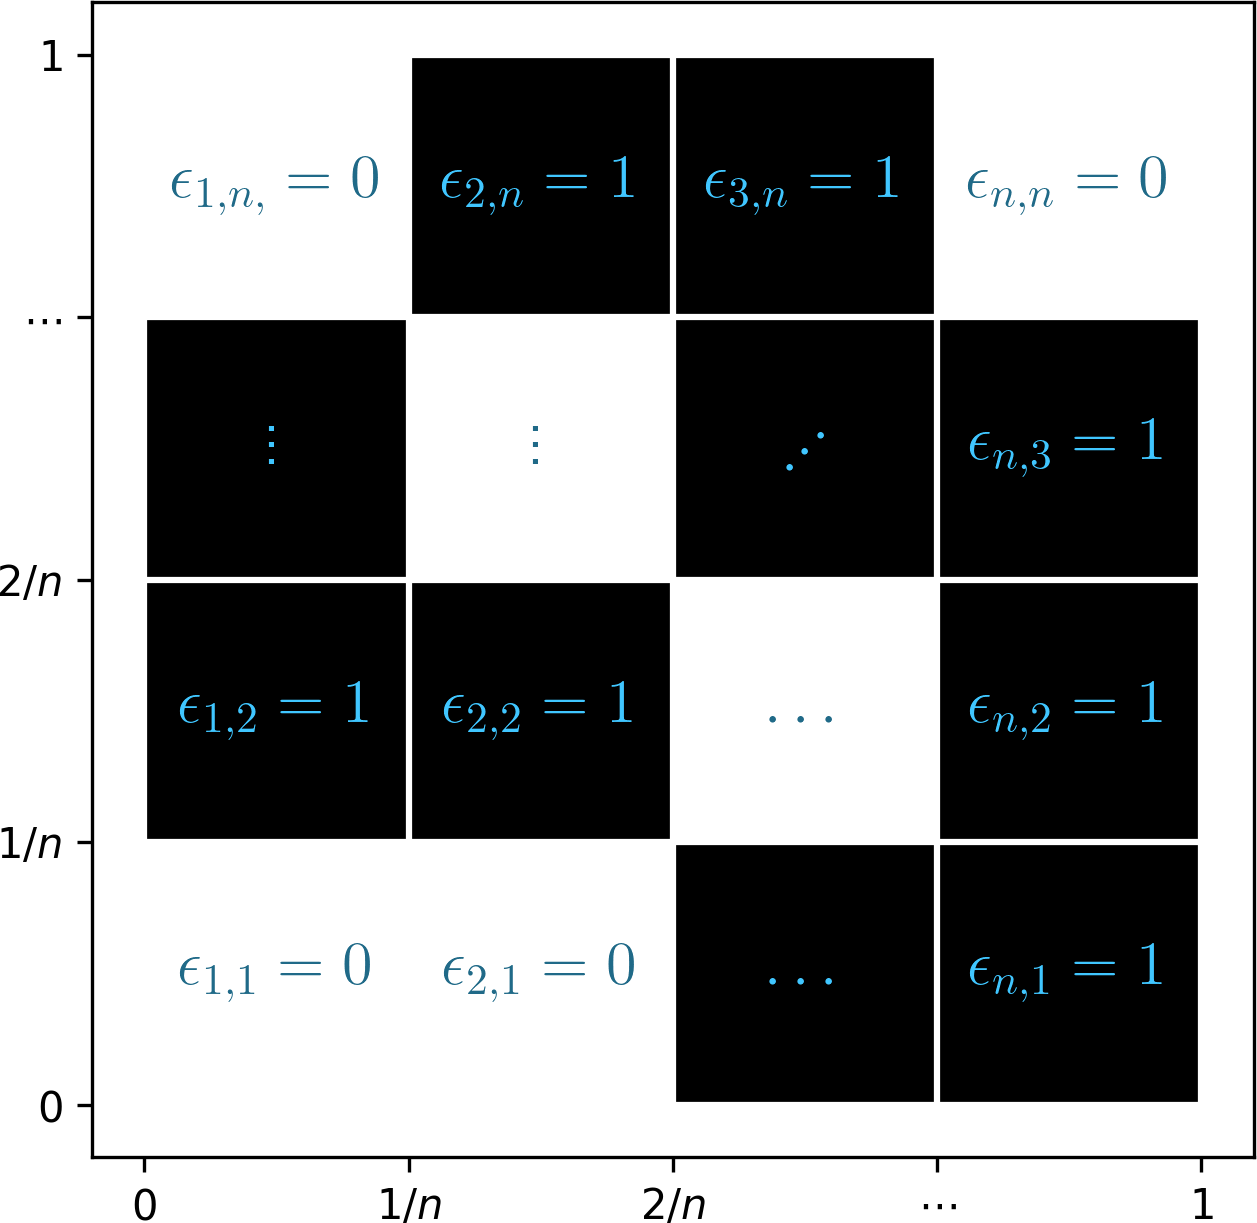
\includegraphics[width=6.5cm]{plain_percolation}
	\caption{Plain Percolation\\($n=4, p=0.6$)}
	\label{fig:plainPercolation}
\end{wrapfigure}
\subsection{Plain Percolation}
The "plain" percolation is the simplest one, as it is only composed of one filtration.
The formal definition goes as follows:
Split the unit square $\left[ 0,1 \right]^2$ into $n^2$ squares of side $\nicefrac{1}{n}$, indexed by $1 \leq i,j \leq n$:
$$B_{i,j} = \left[ \frac{i-1}{n}, \frac{i}{n} \right] \times \left[ \frac{j-1}{n}, \frac{j}{n} \right].$$
Then, each squares will be selected or thrown away, according to random variables $\epsilon_{i,j}$ following a Bernoulli distribution with probability parameter $p$
\footnote{Writing $x \sim \mathcal{B}(p)$ for $x$ following a Bernoulli distribution with parameter $p$, i.e. $\mathbb{P}(x=1)=p$ and $\mathbb{P}(x=0)=1-p$.},
$\epsilon_{i,j} \sim \mathcal{B}(p)$.
Finally, the plain percolation $P$ is
$$P = \bigcup_{i,j \text{ s.t. } \epsilon_{i,j}=1} B_{i,j}.$$

We will adopt the notation $P \sim \text{Perc}(n,p,1)$ for such a setup (a plain percolation of side $n$ and probability parameter $p$).

In this case, it is interesting to study the behaviour as $n \to \infty$, we will write $P \sim \text{Perc}(\infty,p,1)$ for $P = \lim_{n \to \infty} P^n$, $P^n \sim \text{Perc}(n,p,1)$.

\begin{wrapfigure}{r}{7.5cm}
	\vspace{-1.2cm}
	\centering
	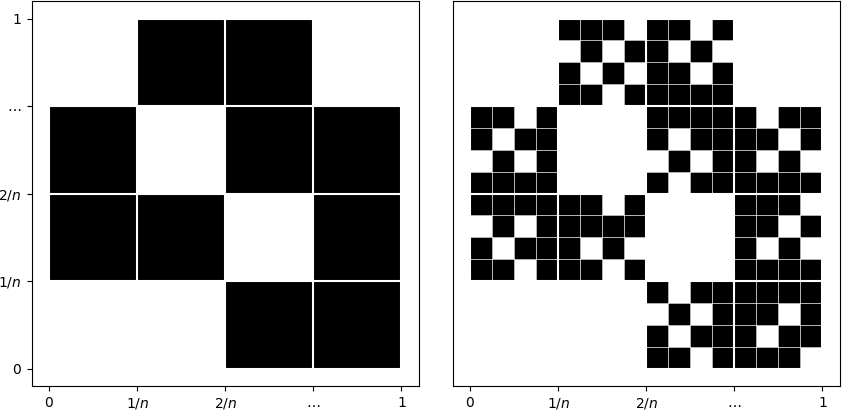
\includegraphics[width=7.5cm]{recursive_percolation_steps}
	\caption{Recursive Percolation\\($n=4, p=0.6, k=1,2$)}
	\label{fig:recursivePercolationSteps}
\end{wrapfigure}
\subsection{Recursive Percolation}
The "recursive" percolation is a little more involved.
Beginning with a plain percolation, we apply an other one to each of the remaining squares, and continue recursively.

Formally, for each $1 \leq k \leq d$, split the unit square into $\left( n^k \right)^D$ squares of side $\nicefrac{1}{n^k}$ indexed by $1 \leq i,j \leq n^k$
$$B_{i,j}^k = \left[ \frac{i-1}{n^k},\frac{i}{n^k} \right] \times \left[ \frac{j-1}{n^k},\frac{j}{n^k} \right].$$
Again, associate to each square a Bernoulli random variable with parameter $p$, $\epsilon_{i,j}^k \sim \mathcal{B}(p)$.
Finally, the recursive percolation $P^d$ is defined recursively by:
$$P^k = P^{k-1} \bigcap \left( \bigcup_{i,j \text{ s.t. } \epsilon_{i,j}^k = 1} B_{i,j}^k \right) \quad \forall 1 \leq k \leq d$$
and $$P^0 = \left[ 0,1 \right]^2.$$

We will adopt the notation $P^d \sim \text{Perc}(n,p,d)$ for such a setup (a recursive percolation of depth $d$, side $n$ and probability parameter $p$).

In this case, it is interesting to study the behaviour as $d \to \infty$, with $n$ fixed.
We will write $P \sim \text{Perc}(n,p)$ for $P = \bigcap_{k \to \infty} P^k$, with $P^k$ defined recursively as above.

\begin{figure}[!h]
	\centering
	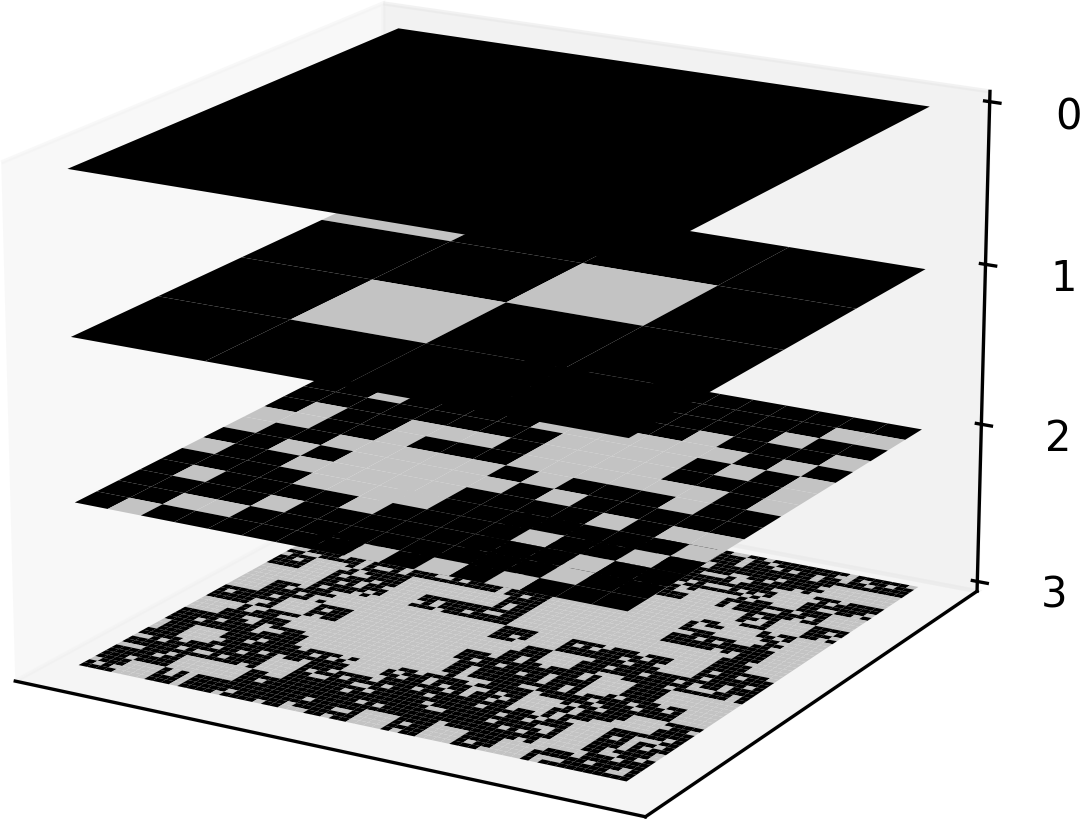
\includegraphics[width=8cm]{recursive_percolation}
	\caption{Recursive Percolation\\($n=4, d=3, p=0.8$)}
	\label{fig:recursivePercolation}
\end{figure}

\subsection{Extension to other dimensions}
Now that we defined percolations in two dimensions, it is straightforward to extend the definition to other dimensions.

\paragraph{Extension to $D$ dimensions}
It suffices to add parameters in the definition to extend it to other dimension, formally:

\subparagraph{Plain}
Split the unit cuboid $\left[ 0,1 \right]^D$ into $n^D$ squares of side $\nicefrac{1}{n}$, indexed by $1 \leq i_1,\dots,i_D \leq n$:
$$B_{i_1,\dots,i_D} = \left[ \frac{i_1-1}{n}, \frac{i_1}{n} \right] \times \dots \times \left[ \frac{i_D-1}{n}, \frac{i_D}{n} \right].$$
Then, attach to each cuboid a Bernoulli random variable $\epsilon_{i_1,\dots,i_D} \sim \mathcal{B}(p)$.
The plain percolation $P$ in $D$ dimension is
$$P = \bigcup_{i_1,\dots,i_D \text{ s.t. } \epsilon_{i_1,\dots,i_D}=1} B_{i_1,\dots,i_D}.$$
%The number of remaining squares $Z$ is $Z = | \{ (i_1,\dots,i_D) \mid \epsilon_{i_1,\dots,i_D} = 1 \} |$.
We will denote this setup by $P \sim \text{Perc}^D(n,p,1)$ (a plain percolation of side $n$ and probability parameter $p$ in $D$ dimensions), and write $P \sim \text{Perc}^D(\infty,p,1)$ for $P = \lim_{n \to \infty} P^n$, $P^n \sim \text{Perc}^D(n,p,1)$.

\subparagraph{Recursive}
For each $1 \leq k \leq d$, split the unit cuboid into $\left( n^k \right)^D$ cuboid of side $\nicefrac{1}{n^k}$ indexed by $1 \leq i_1,\dots,i_D \leq n^k$
$$B_{i_1,\dots,i_D}^k = \left[ \frac{i_1-1}{n^k},\frac{i_1}{n^k} \right] \times \dots \times \left[ \frac{i_D-1}{n^k},\frac{i_D}{n^k} \right].$$
Again, attach to each cuboid a Bernoulli random variable $\epsilon_{i_1,\dots,i_D}^k \sim \mathcal{B}(p)$.
Finally, the recursive percolation $P^d$ is defined recursively by:
$$P^k = P^{k-1} \bigcap \left( \bigcup_{i_1,\dots,i_D \text{ s.t. } \epsilon_{i_1,\dots,i_D}^k = 1} B_{i_1,\dots,i_D}^k \right) \quad \forall 1 \leq k \leq d$$
and $$P^0 = \left[ 0,1 \right]^2.$$

We will denote this setup by $P^d \sim \text{Perc}^D(n,p,d)$ (a recursive percolation of depth $d$, side $n$ and probability parameter $p$ in $D$ dimensions).
And again, we will write $P \sim \text{Perc}^D(n,p,\infty)$ for $P  = \bigcap_{k \to \infty} P^k$, with $P^k$ as above.

In practice, we will never use more than three dimensions.
First, our world is in three dimensions, so it makes sense to stop there.
In addition to that, the curse of dimensionality
%add ref
stops us (calculations and notations are too heavy from the mathematical point of view, and computations are too expensive from a modelling perspective).


\begin{wrapfigure}{r}{6.5cm}
	\vspace{-0.5cm}
	\centering
	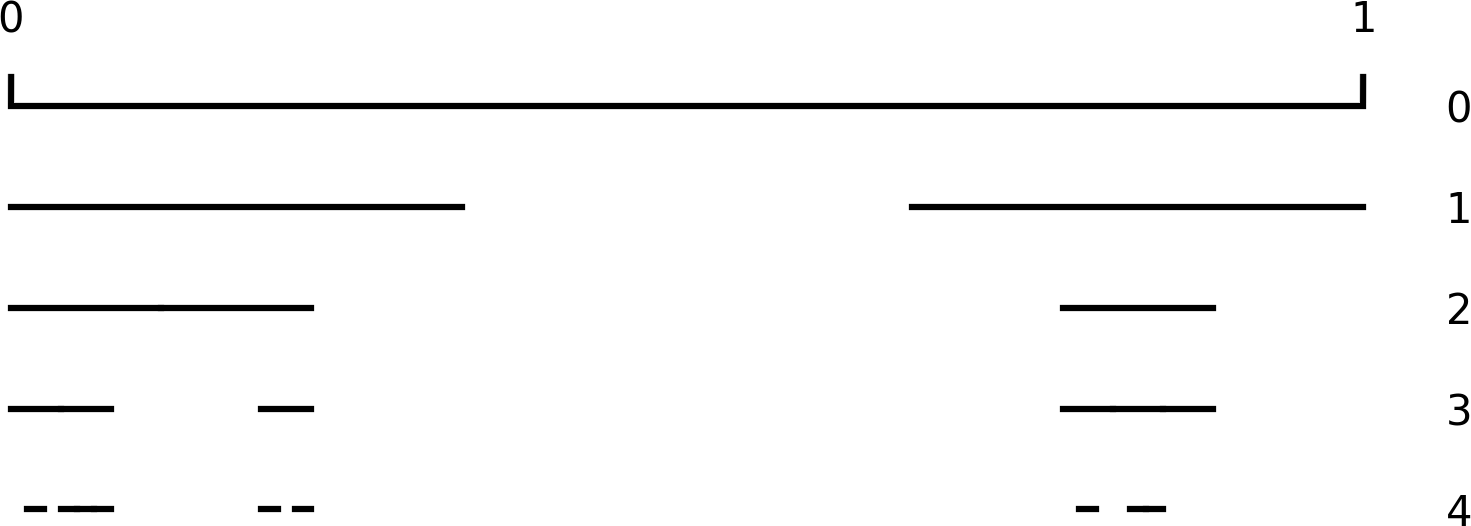
\includegraphics[width=7cm]{Cantor_percolation}
	\caption{1D Recursive Percolation\\($n=3, d=4, p=0.6$)}
	\label{fig:CantorPercolation}
	\vspace{-1cm}
\end{wrapfigure}
\paragraph{Restriction to 1 dimension}
The restriction of the percolation process to one dimension can be though as a randomized and generalized version od the Cantor set.
The Cantor set splits the interval in 3 equal parts, and keep the two extreme ones, while the general recursive percolation process splits the interval into $n$ equal parts, and keep each interval with probability $p$.

\subsection{Density}
Since the percolation process involves randomness, the density is not well defined.
However, it is possible to calculate the expected density
\footnote{The density of a set $X \subseteq \left[ 0,1 \right]^D$ is the proportion of points in the unit cuboid that are also in $X$.}.

It is straightforward to remark that the expected density of a plain percolation $P \sim \text{Perc}^D(n,p,1)$ is $p$ (for all $D$ and all $n$).
Note that this density is constant as $n \to \infty$.

Now, for a recursive percolation $P$ such that $P \sim \text{Perc}^D(n,p,d)$, the density is $p^d$.
Note that this density tends to zero as $d$ grows to infinity (except in the trivial case $p=1$).
Thus, if $P \sim \text{Perc}^D(n,p,\infty)$, the expected density is $0$.

\subsection{Dimensionality}
Again, we can only give an expected dimension, as the process involves randomness.
We ignore the cases $p=0$ and $p=1$ (these are trivial), and we concentrate on $p \in (0,1)$.

We will treat separately the finite cases, and the two limit cases (limit as plain percolation, and as recursive percolation).

\paragraph{Finite Cases}
Take $n$ and $d$ finite, $P \sim \text{Perc}^D(n,p,d)$.
Let $Z$ be the number of remaining squares ($Z = | \{ (i_1,\dots,i_D) \mid \epsilon_{i_n,\dots,i_D} = 1 \} |$).
The expected number of remaining squares is then $\mathbb{E}(Z) = p \left( n^d \right)^D$.

There are two possibilities for the dimension of $P$:
\begin{enumerate}
	\item $Z=0$: then $P = \emptyset$ and dimension of $P$ is $0$;
	\item $Z>0$: then $P \supseteq \left[ \frac{i_1-1}{n^k},\frac{i_1}{n^k} \right] \times \dots \times \left[ \frac{i_D-1}{n^k},\frac{i_D}{n^k} \right]$ for some $(i_1,\dots,i_D)$, so dimension of $P$ is $D$.
\end{enumerate}
Therefore, the expected dimension of $P$ is:
$$
\mathbb{E}(\dim_H(P)) = 0.\mathbb{P}(Z=0) + D.\mathbb{P}(Z>0) = D \left( 1 - \left( 1-p\right) ^{\left( n^d \right)^D} \right).
$$
In practice, this is close to $D$, as soon as $n$ or $d$ grows.
Note that $\dim_T$ would only differ by the fact that $\dim_T(\emptyset) = -1$ whereas $\dim_H(\emptyset) = 0$.
Bow dimension $\dim_B$ will be the same as the Hausdorff one.

\paragraph{Plain Percolation}
We are looking at $P \sim \text{Perc}^D(\infty,p,1)$.
\subparagraph{Heuristic Argument}
Intuitively, the expected dimension of this percolation should be $D$, since the density is positive.
\subparagraph{Formal Calculations}
We show that the Hausdorff dimension is $D$ almost surely.

Let $\mathcal{U}$ be an open cover for $P$, and let $V$ be an open subset of the unit cuboid of dimension $D$.
Then, $\mathbb{P}(P \cap V = \emptyset) = 0$ (as $V$ is uncountable).
Thus, it is almost sure that $\mathcal{U}$ covers $\left[ 0,1 \right]^D$ (otherwise, there is an open subset $V$ of $\left[ 0,1 \right]^D$ not intersecting $P$).
So $H_{\epsilon}^d(P) = H_{\epsilon}^d\left( \left[ 0,1 \right]^D \right)$ almost surely.
Therefore, $\dim_H(P) = \dim_H(\left[ 0,1 \right]^D) = D$ almost surely.

\paragraph{Recursive Percolation}
We are interested in $P \sim \text{Perc}^D(n,p,\infty)$.
\subparagraph{Heuristically}
In the case of a recursive percolation, $P$ has self-similar properties that can help finding the expected dimension.
After the first percolation, each selected cuboid is another version of $P$ scaled by $\nicefrac{1}{n}$.
This goes on recursively.
Therefore, the intuitive dimension to expect is 
$$\mathbb{E}(\dim_H(P)) = \frac{\ln(\mathbb{E}(Z_1))}{\ln(n)}.$$
Where $Z_1$ is the number of remaining cuboids after one percolation $Z_1 = \left| \{ (i_1,\dots,i_D) \mid \epsilon_{i_n,\dots,i_D}^1 = 1 \} \right|$.
So $\mathbb{E}(Z_1) = p n^D$, and finally:
$$\mathbb{E}(\dim_H(P)) = \frac{\ln(p n^D)}{\ln(n)} = D + \log_n(p).$$

\subparagraph{Formally}
The above argument can be made rigorous.
Defining a contractive map that reflects the self similarities;
Then use Stefan Banach's contractive mapping fixed point theorem applied to the complete metric space of non-empty compact subsets of $R^n$ with the Hausdorff distance.

However, we choose to show the fractional dimension is $\alpha = D + \log_n(p)$ directly (this proof follows some ideas from \cite[p. 34-35, ex. 2.7]{Falconer_1990}).

From definition, $P = \bigcap_{d \to \infty} P^k$.
$P^k$ is composed if cuboids of side $\nicefrac{1}{n^k}$.
Let $Z^k$ be the number of these cuboids.
%(i.e. $Z^k = \left| \{ (i_1,\dots,i_D) \mid \epsilon_{i_n//n^{k-j},\dots,i_D//n^{k-j}}^j = 1 \quad \forall j \leq k \} \right|$.
In expectation, $P^k$ should have $\mathbb{E}(Z^k) = \left( p n^D \right)^k$ cuboids of side $\nicefrac{1}{n^k}$ remaining.
Taking $P^k$ as a $\nicefrac{\sqrt{D}}{n^k}$-cover (let $\beta_k = \nicefrac{\sqrt{D}}{n^k}$
\footnote{So that $\beta_k$ is the diameter of a cuboid of side $\nicefrac{1}{n^d}$ in dimension $D$.} ) of $P$ gives 
$$\mathbb{E}\left( H_{\beta_k}^{\alpha}(P) \right) \leq \left( p n^D \right)^k \left( \nicefrac{\sqrt{D}}{n^k} \right)^{D + \log_n(p)} \leq \sqrt{D}^{\alpha}.$$
Letting $k \to \infty$, get
$$\mathbb{E} \left( H^{\alpha}(P) \right) \leq \sqrt{D}^{\alpha} < \infty.$$

%Now, we show that $\mathbb{E} \left( H^{\alpha}(P) \right)  > 0$:
Let $\mathcal{U} = \{ U_i \mid i \in I \}$ be an open cover of $P$.
For each $i \in I$, let $k \in \N$ be such that $\beta_{k+1} \leq \diam{U_i} < \beta_k$.
Then, in general, $U_i$ may only cover one cuboid from $P^k$. As generating $P$ is a random process, it may happen that a $U_i$ covers more than one, but this is not the case in general (as it involves a very particular selection configuration), and will not be consistently the case as we take $k \to \infty$.
Now, if $j \geq k$, then $U_i$ intersects in expectation at most $\left( p n^D \right)^{j-k} \leq \frac{\left( pn^D \right)^j}{\sqrt{D}^{\alpha}} \diam{U_i}^{\alpha}$ cuboids of side $\nicefrac{1}{n^j}$.
Taking $j$ such that $\beta_{j+1} \leq \diam{U_i} \quad i \in I$, since $\mathcal{U}$ intersect in expectation $\mathbb{E}(Z^j) = \left( p n^D \right)^j$ cuboids of diameter $\nicefrac{1}{n^j}$, we get
$$\left( p n^D \right)^j \leq \sum_{i \in I} \frac{\left( pn^D \right)^j}{\sqrt{D}^{\alpha}} \diam{U_i}^{\alpha}.$$
This implies that in expectation, $\sqrt{D}^{\alpha} \leq H^{\alpha}(P)$.
Thus, $\mathbb{E} \left( H^{\alpha}(P) \right)  \geq \sqrt{D}^{\alpha} > 0$.

Finally, as $0 < H^{\alpha}(P) < \infty$, get $\mathbb{E}(\dim_H(P)) = \alpha = D + \log_n(p)$.

\subsection{Blob}
To have a better understanding, we begin by studying the central "blob" of the fractal.
\paragraph{Definition}
We define the blob of a percolation $P$ as the connected component of $P$ that contains the point at the centre of the cuboid (that is, the component that contains $(\nicefrac{1}{2}, \dots, \nicefrac{1}{2})$).
Note that the blob may be empty.

In the simulations, since infinite percolation may only be approximated, we only consider cases where $n$ is odd, so that the cuboid containing the point $(\nicefrac{1}{2}, \dots, \nicefrac{1}{2})$ is uniquely well defined.

\paragraph{Algorithm}
The algorithm we use to find the blob is the following:
%pseudocode?
%strat with the initial middle cuboid
%propagate to all the cuboid of $P$ that are adjacent to one seen before
% wait untill stop!
%% this is the same algorithm idea as the one used in crossing finding, discussed in \reg blah

\subsubsection{Manhattan (step) distance}
%plots and plots comments
\subsubsection{Euclidean distance}
%plots and plots comments
\subsubsection{Area}
%plots and plots comments
\subsubsection{Volume}
%plots and plots comments

\subsection{Random Walks}

